\documentclass{article}

\usepackage[UTF8]{ctex}
\usepackage[utf8]{inputenc} % allow utf-8 input
\usepackage{graphicx}

\title{PA1 Report}
\author{
  计81 包涵 2018011289
}
\date{\today}

\begin{document}
\maketitle

\section{算法实现}
\begin{itemize}
    \item PerspectiveCamera类:按照作业文档中的方法,把相机坐标系中的方向转换为世界坐标系的坐标即可。
    \item Object3D: \begin{itemize}
        \item Group类:使用vector存储objects;在intersect函数中,遍历所有的object并求交,把t值最小的存储并返回。
        \item Plane类:构造函数存储平面的法向量和d值;intersect函数直接求解直线和平面的参数方程。
        \item Sphere类:intersect函数用课件中的方法计算球心到直线的距离,然后计算弦长和t值。
        \item Triangle类:构造函数中计算法向量,虽然mesh.cpp里已经算了;intersect函数先算直线和平面的交点,然后用课件中的方法(Barycentric Technique)判断点是否在三角形内。
    \end{itemize}
    \item Material类:Shade函数实现了作业文档中的Phong模型公式,计算了局部的光强。
    \item main.cpp:实现程序逻辑如下 \begin{itemize}
        \item 从SceneParser中读取Group,Camera和NumLights;从Camera中读取画布尺寸。
        \item 遍历画布的每个像素,生成光线与Group求交,如果相交,再遍历光源,计算该点的光强;不相交则把颜色设成背景。
    \end{itemize}
\end{itemize}

\section{遇到的问题}
\begin{enumerate}
    \item 是否需要normalize的问题:一开始在Ray的构造函数中把输入的参数都normalize了,发现不对,应当由构造函数的调用方保证参数的正确性。
    \item PerspectiveCamera的构造函数:使用了未经初始化的direction参数,导致一部分图片尺寸有问题,改为使用this->direction就解决了问题。
\end{enumerate}

\section{编译运行与结果}
运行run\_all.sh即可编译运行,结果如下\\
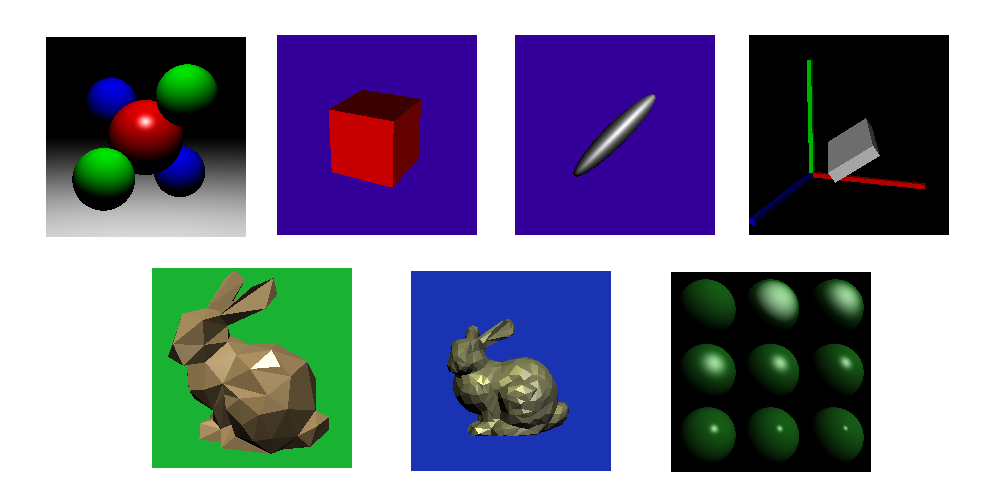
\includegraphics[width=\textwidth]{result.png}

\section{其他}
没有与同学讨论过。目前应该没有bug,但是如果有时间,要实现mesh求交的加速。

\end{document}
